\section{Paper 2}

\title[PhD Defence]{
    {\Huge Paper 2} \\
    \vspace{2mm}
    {\Large Deadline-Miss-Adaptive Controller Implementation} \\
    {\Large for Real-Time Control Systems}
}
\author[Nils Vreman]{
    Nils Vreman \\
    \vspace{3mm}
    {\large Claudio Mandrioli, Anton Cervin}
}
\date[RTAS 2022]{
    Real-Time and Embedded Technology and Applications Symposium, 2022\\
    {\large RTAS Artifact Evaluation - Passed}
}
\notitlelogo
\frame[plain,noframenumbering]{\titlepage}

\begin{frame}
    \frametitle{Co-design}
    \vspace{-1.5cm}%
    \begin{figure}[h]
        \only<1>{\hspace{-2.0cm}\def \delta {0.15}
\def \circlesizecm {0.5cm}
\def \circleshiftcm {0.125cm}
\def \armlength {0.625}
\def \armwidthcm {0.1cm}
\def \bodywidthcm {0.5cm}

\begin{tikzpicture}
\tikzstyle{task} = [draw,thick,fill=white,align=center]
\tikzstyle{turbine} = [circle,ultra thick,draw,fill=white,minimum size=\circlesizecm,inner sep=0pt,outer sep=0pt]

%%% TASKS %%%

\node[task,opacity=0.3] (t1) at (-1.5+0*\delta,1.6-0*\delta) {\textcolor{white}{Task $\#3$} \\\textcolor{white}{\faFileCode[regular]}};
\node[task,opacity=0.6] (t2) at (-1.5+1*\delta,1.6-1*\delta) {\textcolor{white}{Task $\#2$} \\\textcolor{white}{\faFileCode[regular]}};
\node[task,opacity=1.0] (t3) at (-1.5+2*\delta,1.6-2*\delta) {Task $\#1$ \\\faFileCode[regular]};

\node[task,opacity=0.3] (ct1) at (1.5+0*\delta,1.6-0*\delta) {\textcolor{white}{Control Task $\#3$} \\\textcolor{white}{\faFileCode[regular]}};
\node[task,opacity=0.6] (ct2) at (1.5+1*\delta,1.6-1*\delta) {\textcolor{white}{Control Task $\#2$} \\\textcolor{white}{\faFileCode[regular]}};
\node[task,opacity=1.0] (ct3) at (1.5+2*\delta,1.6-2*\delta) {Control Task $\#1$ \\\faFileCode[regular]};

%%% CYBER %%%

\node[thick, align=center] (rtos) at (-0.1,0.25) {Real-Time Operating System};
\node[thick, draw, align=center, rotate=90, text width=2.75cm] (hwi) at (4.1,0.87) {HW Interfaces};
\node[thick, fit=(rtos)(t1)(ct1)(ct3),draw,yshift=1.5mm,xshift=0.75mm] (sw) {};
\node[thick, draw, above left] (clock) at (sw.south east) {\faClock[regular]};
\node[thick, fit=(sw)(hwi), inner sep=7pt, draw] (hw) {};
\node[thick, above left, xshift=2.40cm, yshift=0.5mm] (hw-label) at (hw.south west) {Hardware};
\node[thick, draw, above right] (hwclock) at (hw.south west)  {\faClock[regular]};

%%% PHYSICAL %%%

\node[task, minimum width=2.125cm, minimum height=2.125cm] (phys) at (7.0,0.875) {};
% body
\node[
    draw,
    rounded corners=3pt,
    fill=black,
    minimum width=\bodywidthcm,
    minimum height=\bodywidthcm,
    name path=B] (body) at (phys) {};

% upper left turbine
\node[turbine, anchor=south east] (dronenw) at ([xshift=-\circleshiftcm, yshift=\circleshiftcm]body.north west) {};
\draw[name path=NW] ([yshift=-\armwidthcm]body.north west)..controls($(phys) + (-\armlength, \armlength)$)..([xshift=\armwidthcm]body.north west);
\tikzfillbetween [of=NW and B] {};
\draw[fill=black, rotate=75] (dronenw) ellipse (0.175cm and 0.025cm);
\draw[fill=black, rotate=165] (dronenw) ellipse (0.175cm and 0.025cm);
        
% upper right turbine
\node[turbine, anchor=south west] (dronene) at ([xshift=\circleshiftcm, yshift=\circleshiftcm]body.north east) {};
\draw[name path=NE] ([xshift=-\armwidthcm]body.north east)..controls($(phys) + (\armlength, \armlength)$)..([yshift=-\armwidthcm]body.north east);
\tikzfillbetween [of=NE and B] {};
\draw[fill=black, rotate=75] (dronene) ellipse (0.175cm and 0.025cm);
\draw[fill=black, rotate=165] (dronene) ellipse (0.175cm and 0.025cm);

% lower right turbine
\node[turbine, anchor=north west] (dronese) at ([xshift=\circleshiftcm, yshift=-\circleshiftcm]body.south east) {};
\draw[name path=SE] ([yshift=\armwidthcm]body.south east)..controls($(phys) + (\armlength, -\armlength)$)..([xshift=-\armwidthcm]body.south east);
\tikzfillbetween [of=SE and B] {};
\draw[fill=black, rotate=75] (dronese) ellipse (0.175cm and 0.025cm);
\draw[fill=black, rotate=165] (dronese) ellipse (0.175cm and 0.025cm);

% lower left turbine
\node[turbine, anchor=north east] (dronesw) at ([xshift=-\circleshiftcm, yshift=-\circleshiftcm]body.south west) {};
\draw[name path=SW] ([xshift=\armwidthcm]body.south west)..controls($(phys) + (-\armlength, -\armlength)$)..([yshift=\armwidthcm]body.south west);
\tikzfillbetween [of=SW and B] {};
\draw[fill=black, rotate=75] (dronesw) ellipse (0.175cm and 0.025cm);
\draw[fill=black, rotate=165] (dronesw) ellipse (0.175cm and 0.025cm);

% Clock
\node[task, above left] (time) at (phys.south east) {\faClock[regular]};

%%% ARROWS %%%

\draw[thick, -latex] ([yshift=0.65cm]hwi.south) to node[yshift=0.85cm,xshift=1mm,rotate=90] {Actuation} ([yshift=0.65cm]phys.west);
\draw[thick, -latex] ([yshift=-0.65cm]phys.west) to node[yshift=-0.75cm,xshift=1mm,rotate=90] {Sensing} ([yshift=-0.65cm]hwi.south);

% Requirement
\phantom{\node[align=center, lqgcolour] (req) at (3,3.5) {Requirements dependant\\on the system};}
\phantom{\draw[-latex, thick, lqgcolour] (req) to (ct3);}

%%% CODESIGN %%%

\begin{scope}
    \clip (-5,-1) rectangle (5, 4);
    \phantom{\node[ellipse, draw, thick, lqgcolour, fit=(ct3)] (el-ct3) {};}
    \phantom{\node[ellipse, draw, thick, lqgcolour, fit=(rtos)] (el-rtos) {};}
    \phantom{\draw[latex-latex, lqgcolour, in=180,out=90, thick] (el-ct3.north) to node[left, xshift=-1cm, yshift=-5mm] {Co-Design!} (el-rtos.west);}
\end{scope}

\end{tikzpicture}
}%
        \only<2>{\hspace{-2.0cm}\def \delta {0.15}
\def \circlesizecm {0.5cm}
\def \circleshiftcm {0.125cm}
\def \armlength {0.625}
\def \armwidthcm {0.1cm}
\def \bodywidthcm {0.5cm}

\begin{tikzpicture}
\tikzstyle{task} = [draw,thick,fill=white,align=center]
\tikzstyle{turbine} = [circle,ultra thick,draw,fill=white,minimum size=\circlesizecm,inner sep=0pt,outer sep=0pt]

%%% TASKS %%%

\node[task,opacity=0.3] (t1) at (-1.5+0*\delta,1.6-0*\delta) {\textcolor{white}{Task $\#3$} \\\textcolor{white}{\faFileCode[regular]}};
\node[task,opacity=0.6] (t2) at (-1.5+1*\delta,1.6-1*\delta) {\textcolor{white}{Task $\#2$} \\\textcolor{white}{\faFileCode[regular]}};
\node[task,opacity=1.0] (t3) at (-1.5+2*\delta,1.6-2*\delta) {Task $\#1$ \\\faFileCode[regular]};

\node[task,opacity=0.3] (ct1) at (1.5+0*\delta,1.6-0*\delta) {\textcolor{white}{Control Task $\#3$} \\\textcolor{white}{\faFileCode[regular]}};
\node[task,opacity=0.6] (ct2) at (1.5+1*\delta,1.6-1*\delta) {\textcolor{white}{Control Task $\#2$} \\\textcolor{white}{\faFileCode[regular]}};
\node[task,opacity=1.0] (ct3) at (1.5+2*\delta,1.6-2*\delta) {Control Task $\#1$ \\\faFileCode[regular]};

%%% CYBER %%%

\node[thick, align=center] (rtos) at (-0.1,0.25) {Real-Time Operating System};
\node[thick, draw, align=center, rotate=90, text width=2.75cm] (hwi) at (4.1,0.87) {HW Interfaces};
\node[thick, fit=(rtos)(t1)(ct1)(ct3),draw,yshift=1.5mm,xshift=0.75mm] (sw) {};
\node[thick, draw, above left] (clock) at (sw.south east) {\faClock[regular]};
\node[thick, fit=(sw)(hwi), inner sep=7pt, draw] (hw) {};
\node[thick, above left, xshift=2.40cm, yshift=0.5mm] (hw-label) at (hw.south west) {Hardware};
\node[thick, draw, above right] (hwclock) at (hw.south west)  {\faClock[regular]};

%%% PHYSICAL %%%

\node[task, minimum width=2.125cm, minimum height=2.125cm] (phys) at (7.0,0.875) {};
% body
\node[
    draw,
    rounded corners=3pt,
    fill=black,
    minimum width=\bodywidthcm,
    minimum height=\bodywidthcm,
    name path=B] (body) at (phys) {};

% upper left turbine
\node[turbine, anchor=south east] (dronenw) at ([xshift=-\circleshiftcm, yshift=\circleshiftcm]body.north west) {};
\draw[name path=NW] ([yshift=-\armwidthcm]body.north west)..controls($(phys) + (-\armlength, \armlength)$)..([xshift=\armwidthcm]body.north west);
\tikzfillbetween [of=NW and B] {};
\draw[fill=black, rotate=75] (dronenw) ellipse (0.175cm and 0.025cm);
\draw[fill=black, rotate=165] (dronenw) ellipse (0.175cm and 0.025cm);
        
% upper right turbine
\node[turbine, anchor=south west] (dronene) at ([xshift=\circleshiftcm, yshift=\circleshiftcm]body.north east) {};
\draw[name path=NE] ([xshift=-\armwidthcm]body.north east)..controls($(phys) + (\armlength, \armlength)$)..([yshift=-\armwidthcm]body.north east);
\tikzfillbetween [of=NE and B] {};
\draw[fill=black, rotate=75] (dronene) ellipse (0.175cm and 0.025cm);
\draw[fill=black, rotate=165] (dronene) ellipse (0.175cm and 0.025cm);

% lower right turbine
\node[turbine, anchor=north west] (dronese) at ([xshift=\circleshiftcm, yshift=-\circleshiftcm]body.south east) {};
\draw[name path=SE] ([yshift=\armwidthcm]body.south east)..controls($(phys) + (\armlength, -\armlength)$)..([xshift=-\armwidthcm]body.south east);
\tikzfillbetween [of=SE and B] {};
\draw[fill=black, rotate=75] (dronese) ellipse (0.175cm and 0.025cm);
\draw[fill=black, rotate=165] (dronese) ellipse (0.175cm and 0.025cm);

% lower left turbine
\node[turbine, anchor=north east] (dronesw) at ([xshift=-\circleshiftcm, yshift=-\circleshiftcm]body.south west) {};
\draw[name path=SW] ([xshift=\armwidthcm]body.south west)..controls($(phys) + (-\armlength, -\armlength)$)..([yshift=\armwidthcm]body.south west);
\tikzfillbetween [of=SW and B] {};
\draw[fill=black, rotate=75] (dronesw) ellipse (0.175cm and 0.025cm);
\draw[fill=black, rotate=165] (dronesw) ellipse (0.175cm and 0.025cm);

% Clock
\node[task, above left] (time) at (phys.south east) {\faClock[regular]};

%%% ARROWS %%%

\draw[thick, -latex] ([yshift=0.65cm]hwi.south) to node[yshift=0.85cm,xshift=1mm,rotate=90] {Actuation} ([yshift=0.65cm]phys.west);
\draw[thick, -latex] ([yshift=-0.65cm]phys.west) to node[yshift=-0.75cm,xshift=1mm,rotate=90] {Sensing} ([yshift=-0.65cm]hwi.south);

% Requirement
%\node[align=center, lqgcolour] (req) at (3,3.5) {Requirements dependant\\on the system};
%\draw[-latex, thick, lqgcolour] (req) to (ct3);

%%% CODESIGN %%%

\begin{scope}
    \clip (-5,-1) rectangle (5, 4);
    \node[ellipse, draw, thick, lqgcolour, fit=(ct3)] (el-ct3) {};
    \node[ellipse, draw, thick, lqgcolour, fit=(rtos)] (el-rtos) {};
    \draw[latex-latex, lqgcolour, in=180,out=90, thick] (el-ct3.north) to node[left, xshift=-1cm, yshift=-5mm] {Co-Design!} (el-rtos.west);
\end{scope}

\end{tikzpicture}
}%
    \end{figure}
\end{frame}

\begin{frame}
    \frametitle{Limitations}
    \framesubtitle{Complex \& Conservative Design}
    \begin{figure}
        \centerline{\resizebox{0.65\textwidth}{!}{\begin{tikzpicture}
\tikzstyle{eng-step} = [draw, thick, align=center]


%%% REQUIREMENTS %%%

\node[align=center] (c-req)  at (-3, 2) {Control\\Requirements};
\node[align=center] (rt-req) at ( 3, 2) {Real-Time\\Requirements};

%%% DESIGN %%%

\node[eng-step] (c-des)  at (-3, 0) {Control\\Law\\Design};
\node[eng-step] (rt-des) at ( 3, 0) {Real-Time\\System\\Design};

%%% IMPLEMENTATION %%%

\node[eng-step] (imp)    at ( 0,-2.7) {Control System\\Implementation};
\coordinate[] (above-imp)at ( 0,-1.7) ;
\node[align=center] (out)at ( 0,-4.2) {Software and Hardware\\Product};

%%%%%%%%%%%%%%
%%% ARROWS %%%
%%%%%%%%%%%%%%

\draw[-latex,thick] (c-req)  to (c-des);
\draw[-latex,thick] (rt-req) to (rt-des);
\draw[-latex,thick] (c-des)  to node[above, align=center] (crt-req) {Real-Time Control\\Requirements} (rt-des);

\draw[-latex,thick] (c-des.south)  |- ([xshift=-5mm]above-imp) -- ([xshift=-5mm]imp.north);
\draw[-latex,thick] (rt-des.south) |- ([xshift= 5mm]above-imp) -- ([xshift= 5mm]imp.north);

\draw[-latex,thick] (imp) to (out);

%%% CO_DESIGN %%%

\node[eng-step,dashed,lqgcolour,fit=(crt-req)(c-des)(rt-des)] (co-des) {};
\node[rotate =90, below right, lqgcolour] at (co-des.south east) {Co-Design}; 

\end{tikzpicture}
}}
    \end{figure}
\end{frame}

\begin{frame}
    \frametitle{Limitations}
    \framesubtitle{Increased Runtime}
    \begin{figure}
        \centerline{\resizebox{0.55\textwidth}{!}{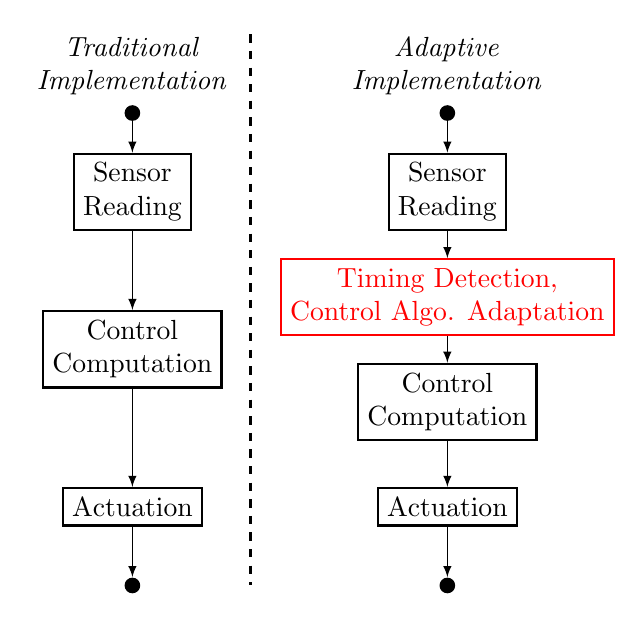
\begin{tikzpicture}
\tikzstyle{block} = [draw, thick, align=center]
\tikzstyle{io-dot} = [circle, fill, inner sep=2pt]

%%% NOMINAL %%%

\node[align=center] ()   at (-2,5.6) {\textit{Traditional}\\\textit{Implementation}};
\node[io-dot](in-nom)    at (-2, 5) {};
\node[block] (sense-nom) at (-2, 4) {Sensor\\Reading};
\node[block] (ctrl-nom)  at (-2, 2) {Control\\Computation};
\node[block] (act-nom)   at (-2, 0) {Actuation};
\node[io-dot](out-nom)   at (-2,-1) {};

\draw[-latex] (in-nom)    to (sense-nom);
\draw[-latex] (sense-nom) to (ctrl-nom);
\draw[-latex] (ctrl-nom)  to (act-nom);
\draw[-latex] (act-nom)   to (out-nom);

%%% INCREASE RUNTIME %%%

\node[align=center] ()   at ( 2,5.6) {\textit{Adaptive}\\\textit{Implementation}};
\node[io-dot](in-cod)    at ( 2, 5) {};
\node[block] (sense-cod) at ( 2, 4) {Sensor\\Reading};
\node[block,red] (tim-cod)   at ( 2, 2.66) {Timing Detection,\\Control Algo. Adaptation};
%\node[align=center, rotate=90] at ( 5, 2.66) {\textit{Perform Optimization (MPC)}\\\textit{re-Computing the controller}};
\node[block] (ctrl-cod)  at ( 2, 1.33) {Control\\Computation};
\node[block] (act-cod)   at ( 2, 0) {Actuation};
\node[io-dot](out-cod)   at ( 2,-1) {};

\draw[-latex] (in-cod)    to (sense-cod);
\draw[-latex] (sense-cod) to (tim-cod);
\draw[-latex] (tim-cod)   to (ctrl-cod);
\draw[-latex] (ctrl-cod)  to (act-cod);
\draw[-latex] (act-cod)   to (out-cod);

\draw[dashed, thick] (-.5,6) to (-.5,-1);

\end{tikzpicture}
}}
    \end{figure}
\end{frame}


\begin{frame}
    \frametitle{Limitations}
    \framesubtitle{Static Controllers}
    \begin{figure}
        \centerline{%
            \begin{tikzpicture}
            \node[align=center,] at (0,1) {Static Controllers:};
            \node[align=center,] at (0,0) {$\mathcal{C}^s : \begin{cases} u_{k+1}=K(r_k-y_k) \end{cases}$};
            \node[align=center,] at (6,1) {Dynamic Controllers:};
            \node[align=center,] at (6,0) {$\mathcal{C}^d :
                                            \begin{cases}
                                                z_{k+1} &= F\, z_k + G\,(r_k-y_k)\\
                                                u_{k+1} &= H\, z_{k} + K\, (r_k-y_k)
                                            \end{cases}$ };
            \end{tikzpicture}}
    \end{figure}

    \begin{figure}
        \centerline{\def \lqr {figs/rtas22a/data/lqr.csv}
\def \lqg {figs/rtas22a/data/lqg.csv}
\def \lqrnom {figs/rtas22a/data/lqr-nominal.csv}
\def \lqgnom {figs/rtas22a/data/lqg-nominal.csv}

\begin{tikzpicture}
    \footnotesize

    %Main axes
    \begin{axis}[%
            height=4.9cm,
            width=\columnwidth,
            xmin=0,
            xmax=5,
            ymin=-0.4,
            ymax=1.1,
            xlabel={Time (s)}, 
            ylabel={Output},
            ytick={-0.4,-0.2,0,0.2,0.4,0.6,0.8,1.0,1.2},
            yticklabels={-0.4,-0.2,0,0.2,0.4,0.6,0.8,1.0,1.2},
            ylabel near ticks,
            grid=major,
            grid style={dashed,black!20},
            legend cell align=left,
            scatter/classes={a={mark=x, mark size=3, color=misscolour}},
            % legend columns = 2
            ]
        
        % LQR-nominal x
        \addplot[lqrnomcolour, very thick ]
                table [x=T, y=X, col sep=comma] {\lqrnom};
        
        % LQR x
        \addplot[lqrcolour, dash pattern={on 3pt off 3pt}, very thick ]
                table [x=T, y=X, col sep=comma] {\lqr};
        
        % LQG-nominal x
        \addplot[lqgnomcolour, very thick ]
                table [x=T, y=X, col sep=comma] {\lqgnom};
                
        % LQG x
        \addplot[lqgcolour, dash pattern={on 3pt off 3pt}, very thick ]
                table [x=T, y=X, col sep=comma] {\lqg};
        
        % Misses
        % scatter src=explicit symbolic gets the scatter definition in axis options.
        \addplot+[scatter, only marks, scatter src=explicit symbolic,thick] coordinates{
            (0.3, -0.4) [a]
            (0.7, -0.4) [a]
            (0.9, -0.4) [a]
            (1.6, -0.4) [a]
            (2.1, -0.4) [a]
            (2.2, -0.4) [a]
            (2.3, -0.4) [a]
            (2.9, -0.4) [a]
            (3.2, -0.4) [a]
            (3.5, -0.4) [a]
            (3.8, -0.4) [a]
            (4.1, -0.4) [a]
            (5.0, -0.4) [a]
        };

        % Legend
        \legend{ Static -- ideal,  Static -- with misses,  Dynamic -- ideal,  Dynamic -- with misses, Overrun};
    \end{axis}

\end{tikzpicture}
}
    \end{figure}
\end{frame}


\begin{frame}{Implementation-Level Approach}
    \begin{minipage}{0.30\textwidth}
        \textbf{Main Assumptions:}
        \begin{itemize}
            \item Deadline miss counter $q$
            \item Kill strategy
        \end{itemize}

        \vspace{1em}

        \textbf{Objective:}
        \begin{itemize}
            \item Increased robustness
            \item Minimal complexity
            \item Minimal overhead
        \end{itemize}
    \end{minipage}\hfill
    \begin{minipage}{0.69\textwidth}
        \begin{figure}
            \centerline{\begin{tikzpicture}
\tikzstyle{eng-step} = [draw, thick, align=center]


%%% REQUIREMENTS %%%

\node[align=center] (c-req)  at (-3, 2) {Control\\Requirements};
\node[align=center] (rt-req) at ( 3, 2) {Real-Time\\Requirements};

%%% DESIGN %%%

\node[eng-step] (c-des)  at (-3, 0) {Control\\Law\\Design};
\node[eng-step] (rt-des) at ( 3, 0) {Real-Time\\System\\Design};

%%% IMPLEMENTATION %%%

\node[eng-step,hicolour] (ada)    at (-3,-1.7) {Control Algo\\Adaptation};
\node[eng-step] (imp)    at ( 0,-2.7) {Control System\\Implementation};
\coordinate[] (above-imp)at ( 0,-1.7) ;
\node[align=center] (out)at ( 0,-4.2) {Software and Hardware\\Product};

%%%%%%%%%%%%%%
%%% ARROWS %%%
%%%%%%%%%%%%%%

\draw[-latex,thick] (c-req)  to (c-des);
\draw[-latex,thick] (rt-req) to (rt-des);
\draw[-latex,thick] (c-des)  to node[above, align=center] (crt-req) {Control Real-Time\\Requirements} (rt-des);

\draw[-latex,thick] (c-des.south)  -- (ada.north);
\draw[-latex,thick] (ada.east)     -| ([xshift=-5mm]above-imp) -- ([xshift=-5mm]imp.north);
\draw[-latex,thick] (rt-des.south) |- ([xshift= 5mm]above-imp) -- ([xshift= 5mm]imp.north);

\draw[-latex,thick] (imp) to (out);

\draw[-latex,thick] (rt-des) to node[above]{$q_{max}$} (ada);

\end{tikzpicture}
}
        \end{figure}
    \end{minipage}
\end{frame}


\begin{frame}
    \frametitle{Experimental Results}
    \centering
    \LARGE
    \textcolor{hicolour}{\url{https://youtu.be/6y\_C7NIzXto}}
\end{frame}

\begin{frame}
    \frametitle{Experimental Results}
    \begin{figure}[h]
        \centering
        \resizebox{0.9\textwidth}{!}{% Set number of bins for histograms in commands file

\begin{tikzpicture}
\begin{groupplot}[group style = {group size = 1 by 4,
                                 vertical sep=0.4cm},
                  width=\textwidth,
                  grid=both,
                  grid style={dashed,black!20},
                  height=3cm,
                  width=\columnwidth,
                  xmin=-5, xmax=2.2,
                  ymin=0, ymax=165,
                  tick align=inside,
                 ]

    %%%%%%%%%%%%%%%
    %%% p = 0.1 %%%
    %%%%%%%%%%%%%%%
    \nextgroupplot[xticklabels = {},
                   legend style = {at = {(0.5,1.1)},
                                   anchor = south,
                                   /tikz/every even column/.append style = {column sep=0.2cm}},
                   legend columns = 3
                  ]
        \addplot[ybar, ybar legend,
                 fill=lqgcolour,
                ] coordinates {(0,0)};
        \addlegendentry{$\ctrler^{n}$}
        \addplot[ybar,
                 hist={bins=\binsaggregatedhist},
                 fill=lqgcolour,
                 forget plot,
                ] 
                table [y index=0, col sep=comma] 
                {\figdir/evaluation/batch-processes/data/batch-results-10-log.csv};
        \addplot[ybar, ybar legend,
                 fill=adacolour,
                ] coordinates {(0,0)};
        \addlegendentry{$\ctrler^{a}$}
        \addplot[ybar, ybar legend,
                 hist={bins=\binsaggregatedhist},
                 fill=adacolour,
                 forget plot,
                ]
                table [y index=1, col sep=comma] 
                {\figdir/evaluation/batch-processes/data/batch-results-10-log.csv};
        % \addlegendentry{$\ctrler^{a}$}
        \addplot[red, dashed, ultra thick] coordinates {(2,0) (2,200)};
        \addlegendentry{Instability threshold}
        \node[draw, fill=white] at (axis cs:1, 125) {$\rho=10\%$};
    
    %%%%%%%%%%%%%%%
    %%% p = 0.3 %%%
    %%%%%%%%%%%%%%%
    \nextgroupplot[xticklabels= {},
                  ]
        \addplot[ybar, hist={bins=\binsaggregatedhist},
                 fill=lqgcolour,
                ] 
                table [y index=0, col sep=comma] 
                {\figdir/evaluation/batch-processes/data/batch-results-30-log.csv};
        \addplot[ybar, hist={bins=\binsaggregatedhist},
                 fill=adacolour,
                ]
                table [y index=1, col sep=comma] 
                {\figdir/evaluation/batch-processes/data/batch-results-30-log.csv};
        \draw[red,ultra thick, dashed] (axis cs:2,0)--(axis cs:2,200);
        \node[draw, fill=white] at (axis cs:1, 125) {$\rho=30\%$};

    %%%%%%%%%%%%%%%
    %%% p = 0.5 %%%
    %%%%%%%%%%%%%%%
    \nextgroupplot[xticklabels= {},
                   ylabel = {Number of systems},
                   ylabel near ticks,
                   ylabel style = {xshift=1cm},
                  ]
        \addplot[ybar, hist = {bins=\binsaggregatedhist},
                 fill = lqgcolour,
                ] 
                table [y index = 0, col sep = comma] 
                {\figdir/evaluation/batch-processes/data/batch-results-50-log.csv};
        \addplot[ybar, hist={bins=\binsaggregatedhist},
                 fill=adacolour,
                ]
                table [y index=1, col sep=comma] 
                {\figdir/evaluation/batch-processes/data/batch-results-50-log.csv};
        \draw[red,ultra thick, dashed] (axis cs:2,0)--(axis cs:2,200);
        \node[draw, fill=white] at (axis cs:1, 125) {$\rho=50\%$};

    %%%%%%%%%%%%%%%
    %%% p = 0.7 %%%
    %%%%%%%%%%%%%%%
    \nextgroupplot[
                   xlabel = {\large$\sfrac{\Delta J^{\dagger}}{J}$},
                   xlabel near ticks,
                  xticklabels = {, $10^{-5}$, $10^{-4}$, $10^{-3}$, $10^{-2}$, $10^{-1}$, $10^{0}$, $10^{1}$, $\infty$,},
                  ]
        \addplot[ybar, hist = {bins=\binsaggregatedhist},
                 fill = lqgcolour,
                ] 
                table [y index = 0, col sep = comma] 
                {\figdir/evaluation/batch-processes/data/batch-results-70-log.csv};
        \addplot[ybar, hist={bins=\binsaggregatedhist},
                 fill=adacolour,
                ]
                table [y index=1, col sep=comma] 
                {\figdir/evaluation/batch-processes/data/batch-results-70-log.csv};
        \draw[red,ultra thick, dashed] (axis cs:2,0)--(axis cs:2,200);
        \node[draw, fill=white] at (axis cs:1, 125) {$\rho=70\%$};

\end{groupplot}
\end{tikzpicture}
}
    \end{figure}
\end{frame}
